\documentclass[12pt]{article} 
\usepackage{amsmath} 
\usepackage[dvips]{graphicx}
\usepackage{multirow} 
\usepackage{geometry} 
\usepackage{pdflscape}
\usepackage{amsmath}
\usepackage[labelfont=bf]{caption} 
\usepackage{setspace}
\usepackage[running]{lineno} 
% \usepackage[numbers,sort]{natbib}
\usepackage[numbers]{natbib} 
\usepackage{array}
\usepackage[table]{xcolor}
\usepackage{xr}

\newcommand{\methods}{\textit{Materials \& Methods}}
\newcommand{\SI}{\textit{Appendix}~}

\topmargin -1.5cm % 0.0cm 
\oddsidemargin 0.0cm % 0.2cm 
\textwidth 6.5in
\textheight 9.0in % 21cm
\footskip 1.0cm % 1.0cm

\usepackage{authblk}


\title{Species motif participation provides unique information about species risk of extinction}

\author{Alyssa R. Cirtwill$^{1*\dagger}$, Anna \r{A}kesson$^{2*}$, Kate L. Wootton$^{3}$, Anna Ekl\"{o}f$^{2}$} 
\date{
\small$^1$Spatial Foodweb Ecology Group\\
Research Centre for Ecological Change\\
Organismal and Evolutionary Biology Research Programm\\
Faculty of Biological and Environmental Sciences\\
University of Helsinki
\medskip
\small$^2$Department of Theoretical Biology, Chemistry, and Physics\\ 
Link\"{o}ping University\\
Link\"{o}ping, Sweden\\
\medskip
\small$^3$ BioFrontiers Institute\\
University of Colorado, Boulder\\
U.S.A.
\medskip
* Joint first authors
\medskip
$^\dagger$ Corresponding author\\
}


\begin{document} 
\maketitle 
\linenumbers
\raggedright

\setlength{\parindent}{15pt} 


\section*{Abstract}


    Bottom-up effects of disturbances to basal resources can strongly affect the persistence of consumers, but it is difficult to predict which species will be most affected by increasing disturbance.
    Coarse measures of a species' structural role, like in-degree and trophic level, are known to affect a consumer's vulnerability to bottom-up disturbance.
    We are interested in whether a richer set of species roles based on participation in three-species motifs is also related to persistence, and how these motif-based roles relate to simpler measures.
    We show that a consumer species' participation in different motifs is related to its probability of persistence. 
    Similarly, the overall motif profile of a network was related to the average persistence of consumer species.
    Notably, we found that networks containing a higher proportion of the `omnivory' motif tend to have lower mean persistence following disturbance, while more frequent participation in the omnivory motif was associated with higher species-level probabilities of persistence.
    Additionally, we find that relationships between motif participation and persistence can synthesize the information provided by in-degree and trophic level.
    Motif participation therefore captures important trends in species persistence and provides a rich description of species' structural roles in their communities.

\begin{spacing}{2.0}

\clearpage
\section*{Introduction} %New

    %\subsection*{1 Why are bottom-up effects important for understanding stability?}
     The plant community is the foundation upon which the myriad species in food webs depend for their survival.
     Disturbances in the plant community have been shown to affect important ecosystem properties such as primary \citep{Hector1999} and secondary production \citep{borer2012plant}, soil respiration and carbon cycling \citep{chen2019plant} and consumer diversity \citep{scherber2010bottom, Baiser2016}.
     As such, the structure of the plant community affects stability across all levels of ecosystem organization, which is crucial for sustaining a healthy energy flow in the ecosystem as a whole~\citep{proulx2010diversity, scherber2010bottom, Rosenblatt2016}. 
     For example, the loss of diversity at the basal level typically causes declines in both abundance and richness of all types of consumers: herbivores, predators, parasitoids, etc. \citep{scherber2010bottom}.


    %\subsection*{2 Global and local network properties are known to affect stability}
    How disturbances, such as population decline or extinction, lead to loss of other species via direct and indirect effects (i.e., secondary extinctions) has for long been vibrant area of research \citep{Santos2021,curtsdotter2011robustness, dunne2009cascading, Eklof2006}.
    Several global (whole-network) as well as local (single-species) properties are known to influence how species respond to disturbances. Two well-known, influential global properties are network size, the number of species present in the network, and network connectance, the number of realized feeding interactions.
    Based on simulations of random networks, large networks were initially thought to be less stable~\citep{May1972}.
    The indisputable presence of large, stable, empirical networks has spurred research into how other structural characteristics, including connectance, may allow large numbers of species to persist~\citep{Dunne2002}.
    Highly-connected networks may be more resistant to secondary extinctions because consumers, on average, have access to a larger number of prey species and can switch from a declining or extinct prey to another resource~\citep{Dunne2002, Eklof2006,Baumgartner2015}. However, a well-connected network also includes more pathways through which a disturbance can spread~\citep{Dunne2004, Vieira2015}. Depending on the strength and arrangements of interactions, this means that species may be impacted through several paths, amplifying the original disturbance and causing more secondary extinctions.
    The net effect of connectance on extinction therefore likely depends on finer-scale (species-level) network structure, as well as the type and severity of disturbance.
    
    
    Species-level properties known to affect species' response to disturbances include trophic level (a measure of the path length between a consumer and a basal resource) and in-degree (number of prey items of a predator). 
    These can also be referred to as local properties of the network.
    Species with high trophic levels (long paths to basal resources) and low in-degree (few prey) are generally at higher risks of secondary extinction \citep{binzer2011susceptibility, Eklof2006}, and disturbances to plant populations cause particularly many econdary extinctions \citep{Curtsdotter2011}. %including secondary extinction due to reduced plant populations.
    However, in-degree and trophic level are both relatively coarse descriptions of a species' role in its food web~\citep{Cirtwill2018FoodWebs}. 
    A more detailed perspective is desirable since, as well as the properties of the consumer itself, a consumer's risk of secondary extinction after a disturbance to plants depends on the extinction risk of its prey.
    For example, a generalist consuming many specialist (and therefore high-risk) prey may be at greater risk of extinction than a specialist which consumes a highly generalist resource that is more unlikely to go extinct (Fig.~\ref{fig:concept}).


    %\subsection*{3 Motif participation may similarly affect species' particular extinction risk}
    It is possible to capture information about how a consumer and its prey fit together within a community by defining participation in different motifs -- unique combinations of small numbers of interacting species~\citep{Stouffer2007,Stouffer2012}. 
    Such motif profiles of species are easily calculated once we know the network structure and require no more information than is used to calculate degree or trophic level.
    These `motif participation' roles capture information about species' direct as well as indirect interactions, incorporating larger-scale network structure into species-level descriptions~\citep{Cirtwill2015a,Cirtwill2018FoodWebs}.
    We refer to these motifs as meso-scale structures to emphasise their role as structures between global (network-level) and local (species-level) properties.  
    A species' motif participation profile shows the second-step indirect interactions the species are affected by, thereby capturing important structures that are missed by global and local properties.  
    Therefore, by allowing researchers to distinguish between, for example, consumers of specialists and generalists, motif participation may complement degree and trophic level to more fully predict species' extinction risk.
    

    While the potential relationships between motif participation and species-level extinction risk have not yet been tested to our knowledge, it has been shown that the frequencies of different motifs within a whole network are associated with community stability \citep{prill2005dynamic, bascompte2005simple} and with changes to the composition of plant communities \citep{giling2019plant}. 
    These relationships between network-level motif frequencies (`motif profiles') and overall community stability mean that a network's motif profile could affect the average extinction risk for consumers within the network.
    Moreover, if network motif profiles are related to average extinction risk, it is worth investigating whether a species' participation in different motifs also affects its extinction risk.

% Severity of disturbance
    As mentioned above, the severity of a disturbance may interact with network structure to affect secondary extinctions.
    A mild disturbance (e.g., leading to a small increase in the probability of basal resources going extinct) is intuitively likely to cause fewer secondary extinctions than a severe disturbance, and the difference in effects can depend on network structure~\citep{Baumgartner2015}.
    Empirical studies have shown that disturbances to plant species can affect some consumers more strongly than others \citep{byrnes2011climate}, that the strength of disturbance affects which consumer species are most strongly affected~\citep{detmer2021variation,carnell2020more}, and that the resilience and return time of the ecological community can be strongly influenced by disturbance severity \citep{rydgren2004disturbance}. 
    The severity of disturbance therefore clearly has an effect on how the ecological community will respond. 

    


%\subsection*{Here we test...}
    Here, we are interested in whether a consumer's extinction risk of going secondarily extinct depends on 1) the motifs in which the species participates, 2) the motif profile of the full food web and 3) the severity of the disturbance to the basal level. %We address this in scenarios with various levels of disturbance targeting the basal level.
    In addition, we want to understand how the information provided by motifs is related to other global and local food web properties in order to better synthesize information provided by different scales of network structure.
    We use synthetic networks and model secondary extinctions using Bayesian networks \citep{Eklof2013, Haussler2020}. 
    As Bayesian networks are computationally efficient (see Methods), we are able to simulate a wide range of disturbance intensities and test whether meso-scale network structure also interacts with severity of the disturbance.
    We focus our analyse on the four network motifs that are over-represented in empirical networks and additionally have been shown to contribute to network stability: the three-species chain, omnivory, apparent competition, and direct competition \citep{Stouffer2007, Borrelli2015a, giling2019plant}.
   
    



\section*{Methods}

    \subsection*{Modelling secondary extinction using Bayesian networks}

        Traditionally, there are two main approaches for studying secondary extinctions. First, there are topological models, based only on food web structure \citep{dunne2009cascading}. Here, extinctions only affect other species in the network once a consumer has lost all of its prey and therefore must go extinct. 
        The second approach uses dynamical models which explicitly simulate population dynamics using a system of differential equations \citep{binzer2011susceptibility}. Dynamical models take changes in prey or predator densities into account when calculating the densities of other species in the network. 
        This additional detail means that realistic processes such as indirect interactions can be included, but also means that dynamical models are highly parameter intensive and simulations are much more time-consuming than topological models. 
        
        
        A middle‐ground approach for simulating secondary extinctions is to use Bayesian networks \citep{Eklof2013,Haussler2020}. 
        In this framework, a consumer's probability of extinction depends on the fraction of resources lost ($f = k/n$ for a species with $n$ resources, of which $k$ have gone extinct) and on a baseline probability of extinction ($\pi$) which captures factors affecting the focal species' extinction probability that are not related to the network structure (e.g., disease, stochastic extinction of small populations).
        Modelling Bayesian networks is fast and computationally efficient, allowing analysis of networks with high species richness \citep{Haussler2020}. 
        This increased speed allows us to simulate a range of disturbance severity rather than single species removals as in many previous studies (e.g.,~\citealp[]{Memmott2004,Staniczenko2010,Dunne2004}).
        Moreover, Bayesian network simulations are less parameter-intensive than dynamical models, meaning that they are less sensitive to assumptions made in the modelling process~\citep{Eklof2013}.
    
        
        The response of the consumer to changes in $f$ can take any form (Appendix \emph{S2}). Here we use a sigmoid non-linear function ($\alpha > 1, \beta > 1$).
		This type of response most accurately captures the secondary extinctions produced by dynamical models (\citealp[]{Eklof2013}).
		The probability of extinction for each species $i$ can therefore be represented using the cumulative density function of a beta distribution:
		\begin{equation}
		P(\lnot i|f) = \pi + (1 - \pi) \frac{B(f;\alpha,\beta)}{B(\alpha,\beta)}.
				\label{betafunc}
        \end{equation}
		
		If all resource species of a consumer \textit{C} are present ($f = 0$), the extinction probability will be $P(\lnot C|f) = \pi$. 
		Similarly, if all resources are extinct ($f = 1$), the extinction probability $P(\lnot C|f)$ will be equal to 1 and the consumer will go extinct.
		If the fraction $f$ is not 1 nor 0, the non-linear sigmoid curve will determine the response of the consumer, which will be more severe if the fraction resources lost is high and less severe if the fraction is small. This will in turn affect the extinction probability $P(\lnot C|f)$.
		For basal resources, we assume that abiotic resources are always available and $f=0$. 
		Following Equation \ref{betafunc}, the extinction probability of a basal resource will only depend on $\pi$.
		Note that we here assume that only the fraction, and not the identity, of the resources lost is important. 
		However, the model can easily be modified to incorporate weighted resource interactions \citep[see][]{Eklof2013}.
		
		
		% how we calculate persistences 
        Beginning with basal resources and working systematically up through the food web, we use Equation \ref{betafunc} to calculate each species' $i$ probability of extinction $P(\lnot i|f)$.
        Using this probability, we then perform Bernoulli trials to determine whether the species goes extinct or not. 
        Species are considered extinct if a random number drawn from a uniform distribution $[0-1]$ is less than $P(\lnot i|f)$.
        These simulated extinctions are used when calculating the fraction of resources lost $f$ for each consumer.
        This allows us to update Equation~\ref{betafunc} with information on extinctions of a focal consumer's resources and simulate bottom-up effects. As this method is probabilistic, we repeat these calculations 100 000 times per network, with unique random draws.
	    For each species, we then define probability of persistence as the fraction of simulations in which the species persists. There are methods for solving Bayesian networks exactly \citep{Eklof2013}.
	    However, for larger networks the described numerical evaluation is highly efficient and produces close to identical results \citep{Haussler2020}.
		
		% BN limitations
		Modelling species extinctions in food webs using Bayesian networks has two main limitations. 
		First, in Bayesian networks consumers do not affect the extinction probabilities of their resources and as such we can here only capture bottom-up effects of disturbances. 
		However, Bayesian networks has been shown to capture the majority of secondary extinctions produced fully-fledged dynamical models \citep{Eklof2013}.
		\cite{Eklof2013} analyzed which functional form of consumers response to loss of resources that most accurately predicted the secondary extinctions realized in the dynamical model, and we here use that functional form in our analyzes.  
		Moreover, bottom-up effects are often the main force of secondary extinctions in empirical systems. 
		For example, bottom-up effects regulate zoo-plankton communities in freshwater lakes, regulating zoo-plankton communities \citep{li2020bottom} and control abundances and biomass of vertebrate species in several terrestrial systems \citep{Dobson2009food, Mduma1999food, Georgiadis2007}. 
		Second, due to the strict bottom-up approach of Bayesian networks the networks must be acyclic.
		Fortunately, \cite{Allesina2009functional} proved that cyclic and acyclic versions of a network have the same properties in terms of secondary extinctions and the effect on network robustness are very limited. 
		Thus, making the networks acyclic in order to use the Bayesian network approach will not strongly affect extinction scenarios.
		Moreover, the cyclic motifs which are excluded from an acyclic network are rare in empirical networks~\citep{Stouffer2007} and therefore unlikely to strongly affect extinction risk.
	
		
    \subsection*{Disturbance scenarios}
    
        In our baseline scenario, all species had an extinction probability of $\pi = 0.1$. 
		To simulate various threats to basal resources, making some species more vulnerable to extinction, we increase basal species' probability of extinction from $0.10$ to $0.5$, in steps of $0.08$. 
		The highest disturbance level, $\pi = 0.5$, corresponds to basal species having a 50\% risk of going extinct. 
		Consumer species retained $\pi=0.1$ in all cases.
		
		
	\subsection*{Initial network construction}

		We generated a realistic set of simulated networks based on the niche model~\citep{Williams2000,Stouffer2007} using the function ``nichemodel'' within the Julia~\citep{Bezanson2017julia} package \emph{BioEnergeticFoodWebs}~\citep{bioenergfw,Delmas2017}. 
		To capture a range of plausible network architectures, we simulated networks with sizes (S) ranging from 50 to 100 species (in steps of 10) and connectances (C) ranging from 0.02 to 0.18 (in steps of 0.04). 
		For full details and a comparison to empirical networks, see \emph{Appendix S1}.
		We removed any biologically unlikely networks (Appendix \emph{S1}) and replaced them with new simulated networks, repeating the process until we obtained 100 suitable networks in each combination of size and connectance.
		To make the simulated networks compatible with the Bayesian simulation framework, all networks were rendered acyclic following~\citet{Allesina2009functional} and species topologically sorted from lowest to highest trophic level (Appendix \emph{S1}). 
		 These processing steps allow the strictly bottom-up calculation of probability of persistence.
		
		
	\subsection*{Defining species roles}

        A species' ``motif participation role'' is the frequency with which a focal species appears in each of the motifs present in a network~\citep{Stouffer2012}.
        In our case, these are four-dimensional vectors since only four three-species motifs can appear in acyclic networks.
        As we are interested in relationships between the type of motif participated in rather than the total number of motifs, we normalized participation vectors by dividing each count by the total number of motifs the species appears in.
        Note, however, that this normalization does not necessarily control for differences due to degree or connectance as high- and low-degree species (or species in more- and less-connected networks) may also tend to participate in different types of motifs.
        We address the potential associations between motif participation, degree, and connectance explicitly below. 
        
        
        To provide context for species' motif participation, we also calculated network ``motif profiles'': four-dimensional vectors of the number of each three-species motif in each network~\citep{Stouffer2012}.
        To separate differences in motif structure from differences in network size (larger networks contain more motifs), we normalized motif profiles by dividing the count of each motif by the total count of all motifs. 
		We calculated species' motif participation using the Python package \emph{pymfinder}~\citep{pymfinder}.


        Finally, we calculated simpler measures of a species' role within its community.
        These were in-degree (number of prey) and trophic level (shortest trophic level (STL): the length of the shortest food chain between the focal species and any basal resource~\citep{Williams2004}).
        Both simple role measures were calculated in R~\citep{R} using the same algorithm as~\citet{Eklof2013}.
        


	\subsection*{Statistical analysis} 
	% Appendix 3, with numbered subheadings.

    	We tested 1) how species persistence varied with motif participation, 2) how motif participation varied with other network properties (in-degree and trophic level, STL), 3) how network mean persistence (the average persistence of all consumers in the network) varied with network motif profiles, 4) how network motif profiles varied with global structural properties (S and C), and 5) how species persistence and network mean persistence varied with other network properties (S, C, in-degree, and trophic level).
        Where applicable, we also consider how interactions between network structure and disturbance level might affect extinction risk.
    	See Appendix \emph{3.1 - 3.5} for details. 
    	All analyses are briefly described below and were performed using the R~\citep{R} packages \emph{lmerTest}~\citep{lmerTest}, \emph{MuMIn}~\citep{MuMIn}, and \emph{vegan}~\citep{vegan}.

        
        \subsubsection*{1) Species persistence and motif participation}

            To test if participating more often in a certain motif affected a species' probability of persistence, we fit four linear mixed-effect models (LMMs; one per motif included in the Bayesian networks):
                \begin{equation}
                    \Psi_{ink} \approx \rho_{i} + \pi_{k} + \rho_{i}\pi_{k} +
                    S_{n}C_{n} + N_n,
                    \label{propreq}
                \end{equation}
            \noindent where $\Psi_{ink}$ is the persistence of species $i$, belonging to network $n$, during disturbance level $k$, $\rho_{i}$ is the proportion of the role of species $i$ that is made up by the focal motif, $\pi_k$ is the probability of extinction for a basal resource in disturbance level $k$,  $S_{n}C_{n}$ is a random intercept for the species richness and connectance of network $n$, and $N_n$ is a random effect of network $n$, intended to account for the non-independence of motif participations for species in the same network.
            All predictors were centered and scaled before fitting the models.         
            To test whether these general trends were consistent across networks, we visually examined the distribution of slopes of simplified regressions fit to a single network and level of disturbance (Appendix \emph{3.1}).
        
        \subsubsection*{2) Motif participation and other network properties}    
            
            Properties which refer to different scales of network structure, including different amounts of direct and indirect interactions with the focal species, are not independent. 
            To identify correlations between global network structure (i.e., the whole network) and participation in particular motifs (a meso-scale description of species roles), we fit a series of LMs relating motif participation to network size, connectance, and their interaction (Appendix \emph{S3.2}).
            We fit a similar set of  LMMs relating motif participation to in-degree or trophic level (i.e., local measures of a species' role; Appendix \emph{S3.2}).
            Taken together, these supplemental models demonstrate how motif participation relates to other measures of network structure.
            
            
        \subsubsection*{3) Network mean persistence and motif profiles}

            As well as species-specific probabilities of persistence, the overall frequency of motifs in a network may provide information about the overall probability of any species going extinct (since they incorporate information on indirect effects).
            We tested whether networks with similar motif profiles tend to have similar mean persistences among consumers using a PERMANOVA (Appendix \emph{S3.3}).
            To identify the relationships between particular motifs and network mean persistence in more detail, we fit a set of four LMs (one per motif):
                \begin{equation}
                    \overline{\Psi_{nk}} \approx \Bar{\rho}_{n} + \pi_{k} + \Bar{\rho}_{n}\pi_{k},
                    \label{netpropeq}
                \end{equation}
            \noindent where $\overline{\Psi_{nk}}$ is the mean persistence of all consumers in network $n$ at disturbance level $k$, $\Bar{\rho}_{n}$ is the proportion of the focal motif in the network's motif profile, and $\pi_k$ is the level of disturbance (probability of extinction for basal resources) as in equation~\ref{propreq}.
                
        \subsubsection*{4) Motif profiles and network properties}
        
            To test whether networks with the the same size and connectance have more similar motif profiles, we used a PERMANOVA~\citep{Anderson2001} of Bray-Curtis dissimilarity among motif profiles against network size, connectance, and their interaction (Appendix \emph{S3.4}). 
            In addition, we identify correlations between size, connectance, and particular motifs using a set of four LMs:
            \begin{equation}
                \Bar{\rho_{n}} \approx \Sigma_{n} + \zeta_{n} + \Sigma_{n}\zeta_{n}
            \label{profile_global}
            \end{equation}
            \noindent where $\Bar{\rho}_{n}$ is the proportion of the focal motif in the motif profile of network $n$ and $\Sigma_n$ and $\zeta_{n}$ are the size and connectance of network $n$.
            
        \subsubsection*{5) Persistence and network properties}
            
            Persistence is known to vary with global-scale and local-scale network properties.
            To correctly interpret any relationships between motifs and persistence, we must consider the context of these other relationships (Appendix \emph{S3.5}).
            To identify the relationship between global network structure and mean probability of persistence within a network, we fit a linear regression relating mean persistence to network size, connectance, disturbance, and their interactions (Eq. S9).
            As the three-way interaction was significant, we did not simplify the model. 


            Persistence is also known to vary with local-scale measures of network structure. 
            To identify the relationships between local-scale properties and species' probabilities of persistence, we fit two final LMMs relating a consumer's persistence to disturbance, in-degree or STL, and the interaction between disturbance and the local-scale measure (Eq. S10-S11).
            These LMMs also included random effects to account for the effects of global network structure and network ID on persistence.


\section*{Results}

    \subsection*{Species persistence and motif participation} 
    % Coefficients changed slightly with network-level random effect, but conclusions similar
       The relationship between frequency of participation in a motif and a species' probability of persistence depended on the level of disturbance. 
       When disturbance ($\pi$) was low, species' persistence increased with increasing proportions of the omnivory and direct competition motifs. 
       Conversely, persistence decreased with an increasing proportion of the apparent competition motif. 
       Persistence was not significantly related to the proportion of the three-species chain motif (Figure~\ref{fig:prop_lmer_all}; upper lines in each panel).
            
            
        At high levels of disturbance, a species' persistence decreased as the proportion of the three-species chain in its motif profile increased.
        Persistence increased as the proportion of any other motif increased (Figure~\ref{fig:prop_lmer_all}; lower lines in each panel). 
        This means that increased disturbance strengthened the effects of the three-species chain motif and changed the direction of the effect of the apparent competition motif  (Figure~\ref{fig:prop_lmer_all}, Table S1, \emph{Appendix S4}).
        The relationship between omnivory and persistence was still positive but weaker at higher levels of disturbance, and the relationship between persistence and direct competition was largely unaffected by disturbance.

    \subsection*{Motif participation and other network properties}
        % Updated with network-level random effect. No visible change.
        Species' motif participation varied depending on the global properties of the network: size, connectance, and their interaction (Fig. S1, Table S2; \emph{Appendix S5}).
        Species appeared most often in the apparent competition motif in all types of networks, but the proportion of apparent competition decreased with increasing network size and connectance.
        The proportion of the omnivory motif in a species' participation role increased sharply with increasing connectance, while the proportion of the direct competition motif increased slightly with increasing network size. 

        % Updated with network-level random effect. No visible change.    
        Species' motif participation also varied with their in-degree and trophic level (Fig.~\ref{fig:motifs_vs_TL_and_deg}).
        Species with higher in-degree tended to have higher frequencies of participation in the omnivory motif. Proportions of the other three motifs tended to decline with increasing degree.
        Species with higher trophic levels tended to have higher proportions of apparent competition and three-species chains. 
        % Updated with network-level random effect. No visible change.   
        A species' persistence varies with both species in-degree and trophic level (Fig.~\ref{fig:motifs_vs_TL_and_deg}; \emph{Appendix S6}). 
        Increased trophic level is generally associated with decreasing species persistence, although the rate of decline is slower at high disturbance (Table S3, \emph{Appendix S6}).
        In-degree shows an even stronger interaction with disturbance; having more prey species is associated with higher persistence without disturbance, but lower persistence at high levels of disturbance.
        
        
        \subsubsection*{Consistency in effects of motif participation on species persistence}
    
            %Update not needed
            When fitting regressions of persistence against motif participation for each network separately, networks with high connectance generally showed more consistent relationships between persistence and motif participation, i.e., sharper peaks of the density distributions (Fig.~\ref{fig:density_prop_C}).
            However, this trend varied at different levels of disturbance, especially for the direct competition and omnivory motifs.
            At low and medium connectances there was little change in the distribution of slopes for direct competition across all levels of disturbance. 
            At high connectances, however, the proportion of positive slopes was both lower overall and decreased with increasing disturbance. 
            For the omnivory motif these trends were reversed. 
            Moreover, the omnivory motif has a particularly broad distribution of slopes (i.e., an inconsistent relationship to persistence) when network connectance was low. 
            Network size had a much smaller effect than connectance (Fig. S4; \emph{Appendix S7}).


    \subsection*{Network mean persistence and motif profiles}
        % Updated to use means instead of all species
        The overall motif profile of a network was related to the average persistence of consumers ($F_{1,2998}$=645, $p$\textless0.001), although this result must be considered tentative due to non-homogeneous distribution of roles (\emph{Appendix S8}). 
        Average persistence was higher in networks with higher proportions of the three-species chain, direct competition, and apparent competition motifs (Table S4, \emph{Appendix S8}). 
        Conversely, average persistence was lower in networks with higher proportions of the omnivory motif. 
        These trends were consistent across levels of disturbance (Fig.~\ref{fig:motif_profile_persistence}, Table S4), \emph{Appendix S8}).% Network persistence varies between networks with different dispersion of motif profiles ($F_{134,2865}$=2.19$\times10^{24}$, $p$=\textless0.001). For example, networks with more variable motif profiles have higher persistence ($\beta$=0.183, $p$\textless0.001).


    \subsection*{Motif profiles and network properties}

        Although the PERMANOVA test relating overall motif profiles to network properties was not reliable (Fig. S5, \emph{Appendix S9}), 
        connectance was significantly related to the frequencies of different motifs in a network when considering motifs individually (Fig.~\ref{motif_proportion_lms}).
        Network size and the interaction between network size and connectance did not strongly affect the frequencies of most motifs.
        Considering each motif separately, the proportions of apparent competition and three-species chains in a network's motif profile tended to decrease with increasing connectance while the proportion of omnivory increased with increasing connectance (Table S5, \emph{Appendix S9}). 
    


% Appendices SA (persistence vs. S,C), SH-I (analyses with motif positions), SJ-K (repeated analyses with number of basal resources instead of disturbance) not referred to in text. Keeping SH-K in commented-out form in case reviewers ask. We should refer to SA somewhere in Discussion (will be Appendix 10).


\section*{Discussion}

    The effects of bottom-up disturbances on consumers depend on the global structure of the affected food web~\citep{Dunne2002, Eklof2006, PascualDunne2006}.
    Likewise, the distribution of meso-scale structures within a network affects the network's stability~\citep{prill2005dynamic, bascompte2005simple}.
    In addition, both direct and indirect interactions (i.e., the local and meso-scale structure of a food web  [\citealp[]{Cirtwill2018FoodWebs}]) can affect which species are most strongly affected~\citep{curtsdotter2011robustness, dunne2009cascading, Eklof2006}. 
    Identifying these species is a high priority for conservation efforts~\citep{Bottrilletal2008}.
    To advance this goal, we systematically explore the relationships between meso-scale structures and species' extinction risk, as well as how these trends overlap with the effects of global- and local-scale network properties.

    
    % Species-level results summary
    A species' frequent participation in the direct competition and omnivory motifs was associated with a higher probability of persistence while participation in the three-species chain motif was associated with lower persistence, regardless of the strength of disturbance.
    The strength of disturbance strongly affected the relationship between persistence and participation in the apparent competition motif.
    These trends can be partially explained by underlying relationships between motif participation and local-scale network properties.
    For example, species with higher trophic levels tended to participate less often in the direct competition motif.
    A high trophic level is always associated with lower persistence since predators necessarily have lower probabilities of persistence than their prey~\citep{Eklof2013}.
    Accordingly, high participation in the direct competition motif, by indicating a low trophic level, is associated with high probability of persistence.
    
    
    % Degree and TL are both important for omnivory
    The relationship between participation in the omnivory motif and persistence connects motif participation with both in-degree and trophic level (STL).
    Species participation in the omnivory motif was associated with greater persistence, especially at low levels of disturbance.
    This is consistent with a strong negative correlation between omnivory and trophic level (leading to the overall positive effect of omnivory) and a strong positive correlation with in-degree (leading to the reduced benefit of omnivory at high levels of disturbance). 
    Motifs can thus act as a tool for synthesizing the information provided by other measures of a species' place in its community and for understanding the interactions among these measures.
    
    
    % Degree and TL don't explain everything
    The relationships between persistence and participation in the apparent competition and three-species chain motifs likewise demonstrate the potential for motif participation to synthesize different aspects of network structure.
    In these cases, in-degree and trophic level are not sufficient to explain the trends we observe in the motifs.
    For apparent competition, there were strong and opposing correlations with in-degree and trophic level but the relationship between apparent competition and persistence only matches the trends for in-degree.
    This suggests that some other factor is over-riding the relationship between apparent competition and trophic level.
    
    
    Similarly, participation in the three-species chain motif was significantly correlated with both in-degree and trophic level, but the relationship between motif participation and persistence did not reflect the disturbance-dependent relationship between in-degree and persistence.
    This suggests that the relationship between persistence and participation in the chain motif synthesizes the effects of in-degree, trophic level, and some additional effect which counterbalances the effect of in-degree.
    This additional effect may come from indirect interactions, which are described by motifs but not in-degree~\citep{Cirtwill2018FoodWebs}. 
    
    
    % Moving to network context
    As well as clarifying the relationships between network structure and the effect of bottom-up disturbance on particular species, motifs were also related to the mean probability of persistence across all species in a network.
    In fact, a network's motif profile had a stronger relationship to mean persistence compared to both network size and connectance. 
    This suggests that network motif profiles may be more useful than global network properties when predicting mean extinction risk of species in a network.
    Connectance did, however, affect which motifs were most common within a network. 
    Highly-connected networks tended to contain higher frequencies of the omnivory motif, which includes more links than the other three-species motifs considered here.
    Global-scale properties may therefore indirectly affect network persistence by changing meso-scale properties, such as the distribution of motifs. 
    
    
    In general, average persistence was highest in networks with low proportions of the omnivory motif and high proportions of the apparent competition motif. 
    These results contrast with earlier work showing that higher numbers of omnivory motifs and lower numbers of apparent competition motifs are associated with greater food-web persistence~\citep{Stouffer2010b}.
    By using counts of motifs rather than proportions,~\citet{Stouffer2010b} may be mixing effects of total numbers of motifs with effects of motif proportions.
    Moreover, the effect of omnivory on stability is known to be highly context-dependent \citep{bascompte2005simple, Monteiro2016,McLeod2021}. 
    The stability of omnivory motifs in isolation depends on the strength of the omnivore-resource interaction~\citep{McLeod2021}, but at the whole-network level interactions with other species can stabilize even intrinsically unstable omnivory \citep{Kratina2012}. 
    This might be why we find different patterns between a network's motif profile (where a high proportion of omnivory indicates lower average network persistence) versus a single species motif participation (where a high proportion of the omnivory motif indicates a higher focal species persistence).
    Thus, the ideal situation appears to be being a highly omnivorous species in a low-omnivory setting. 
    
    % High C webs and omnivory
    Supporting this possibility, species participate more frequently in the omnivory motif in high-connectance networks and the relationship between persistence and participation in the omnivory motif is more strongly positive (Fig.~\ref{fig:density_prop_C}) as in~\citet{McLeod2021}.
    These networks contain many pathways by which a bottom-up disturbance can propagate through the network, leading to stronger effects of disturbance on consumers (Table S6; \emph{Appendix S10}).
    In such a network, it may be especially beneficial for a species to feed on multiple trophic levels and, in a sense, spread its risk of losing prey to bottom-up effects.
    Although species in our model cannot swap prey, the reduced extinction risk for omnivorous species resembles empirical studies showing that adaptive omnivory can increase the permanence of three-species chains~\citep{Fagan1997, Kvrivan2005, AbramsFung2010}.
    
    
    There are limitations to the approach presented here.
    Most importantly, the Bayesian network framework operates on a strict bottom-up principle and therefore cannot include top-down effects in the extinction risk calculations~\citep{Eklof2013}. 
    Here our focus was to analyze the importance of disturbances to the basal resources, in which case the Bayesian network approach captures a majority of the secondary extinctions obtained in a fully-fledged dynamical model with much greater efficiency~\citep{Eklof2013}.
    If top-down effects are important for a particular empirical system, however, our simulations may not be accurate. 
    Ongoing work using a dynamical model shows that time to extinction for species following disturbance is tightly coupled to the motifs a species participates in, and that adding top-down effects can lead omnivory to be negatively correlated with persistence \citep{Cirtwill2021_inprep}. 
    If top-down effects are not crucial, the Bayesian network approach could be extended by explicitly incorporating information on species traits.
    In empirical webs, species traits are related to both motif participation~\citep{cirtwill2018feeding} and extinction risk~\citep{Brose2017, curtsdotter2011robustness, Cardillo2005, Purvis2000},
    adding an extra dimension of information which we do not consider here.
    
    In summary, our results show that participating in different three-species motifs is related to a species' risk of extinction following a bottom-up disturbance, and that these relationships synthesize information provided by other, simpler measures of species roles.
    Critically, our results also underscore the importance of considering the level of disturbance when identifying which species are most at risk of extinction.
    There were strong interactions between the level of disturbance and the relationships between persistence and multiple measures of species roles (motifs and in-degree).
    These simulated results echo other warnings about `tipping points' where previously beneficial traits can become risky~\citep{Latty2019,Golubski2016,Tylianakis2014}.
    For example, at low levels of disturbance a high degree may be protective since species can compensate if one or a few prey are lost. 
    At high disturbance, however, a high-degree species is likely to be affected by disturbances through many paths and have lower persistence.
    These disturbance effects mean that efforts to define a set of target species for conservation interactions must take the current (and future) level of disturbance the community experiences into account.
    
\section*{Acknowledgements}

    The authors thank György Barabás for excellent discussion of the ideas in this manuscript. AÅ is supported by the Swedish Research Council for Sustainable Development Formas (\#2015-01262) granted to AE. ARC is supported by a Finnish Academy postdoctoral research grant (\#332999).

\clearpage    

\section*{Figures}
    
 %   \begin{figure}[hb!]
 %      \centering
 %       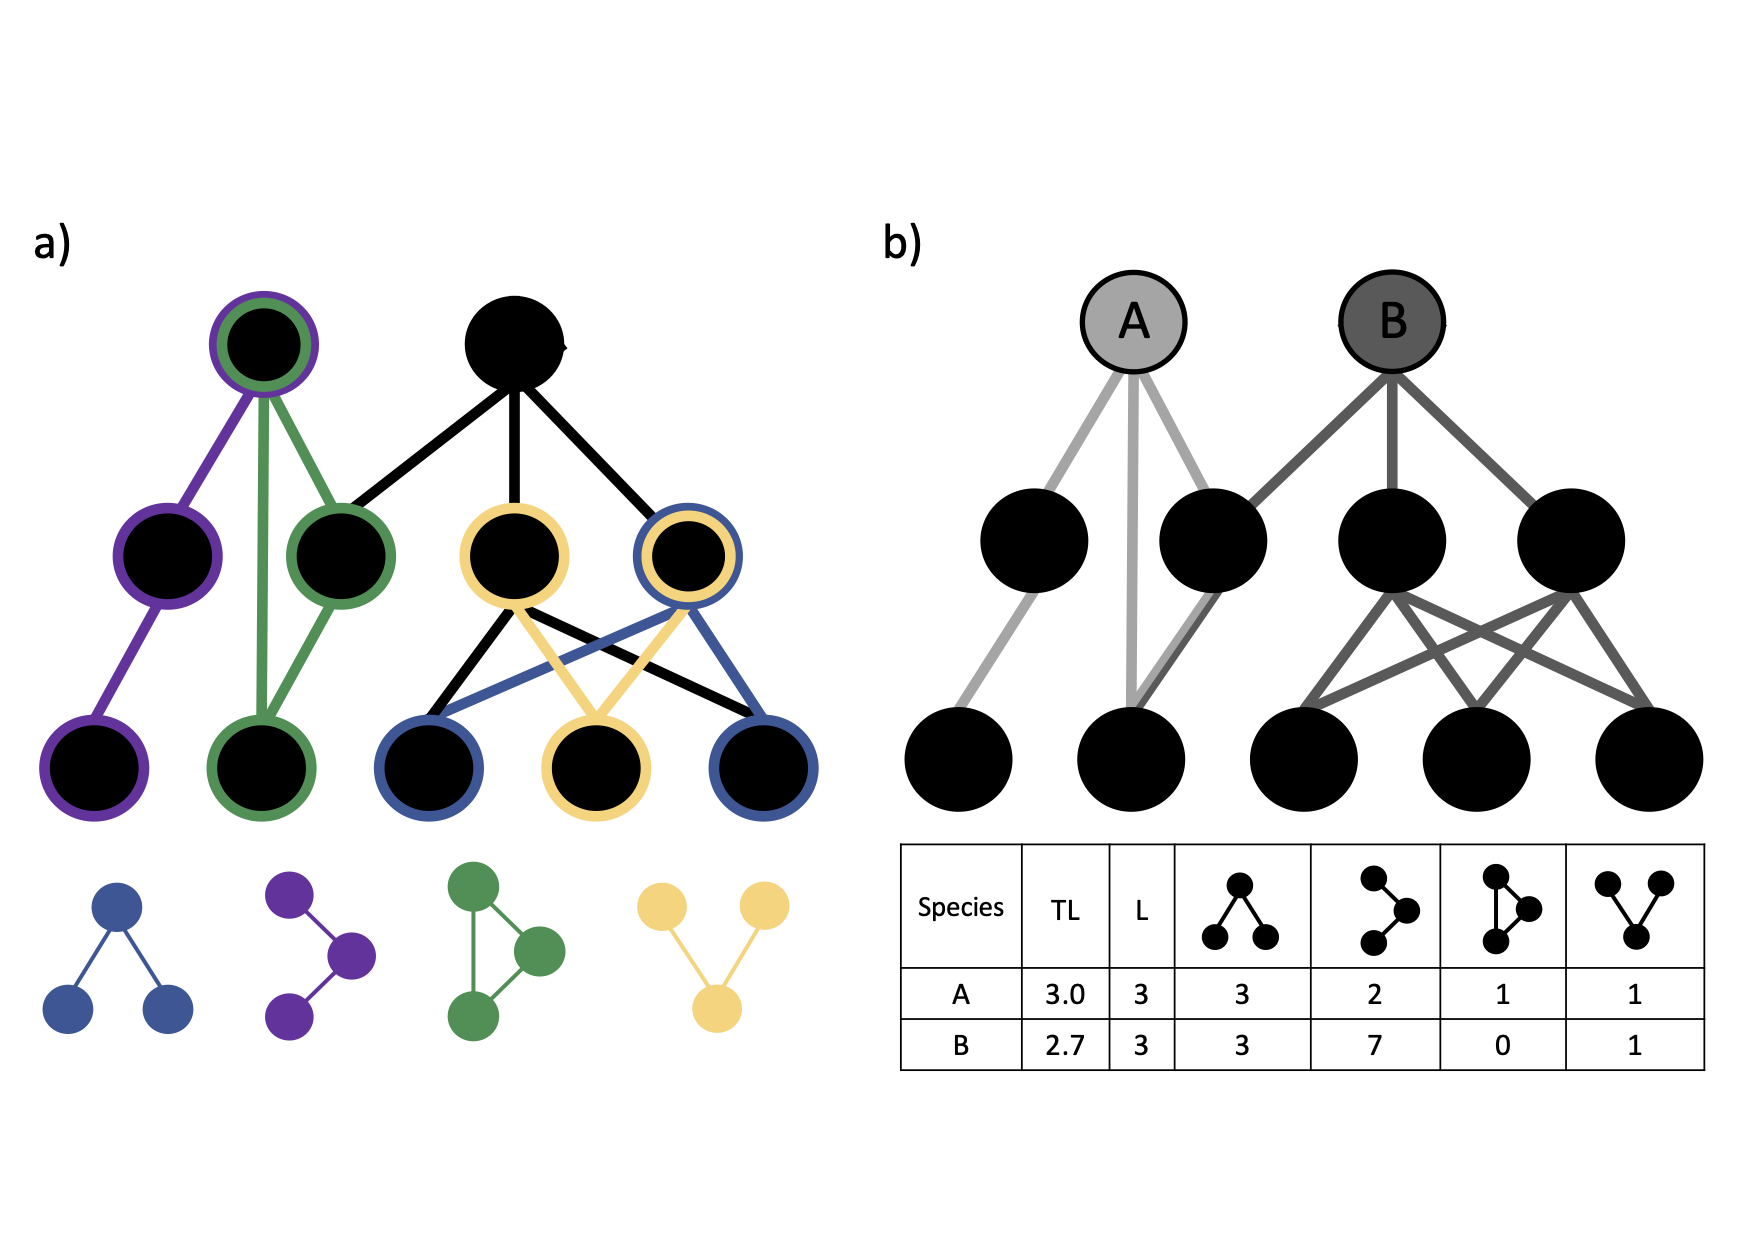
\includegraphics[width=1.0\textwidth]{manuscript/figures/concept_motifs_ab.png}
 %       \caption{Conceptual figure of a toy food web. \textbf{a)} This web contains examples of the four motifs present in an acyclic Bayesian network: apparent competition (blue), three-species chain (purple), omnivory (green), and direct competition (yellow). These motifs capture different ways in which disturbances to basal resources can propagate through the network. For example, a disturbance to the bottom species in a three-species chain will have a direct effect on the middle species but only indirectly affect the top species while a disturbance to the bottom species in an omnivory motif will have a direct effect on the middle species and direct and indirect effects on the top species. Note that the nodes participate in more motifs than the ones highlighted. \textbf{b)} In the same food web, species with similar degree and trophic level can have different motif participation; here species A (light grey node with links in the same motif colored light grey) participates in only two chains while species B (dark grey node with its direct consumption links colored dark grey) participates in chains more than tree times more frequently. Inserted table shows the number of times A and B, respectively, participate in the four different motifs.}
 %   \label{fig:concept}
 %   \end{figure}
    
        \begin{figure}[hb!]
        \centering
        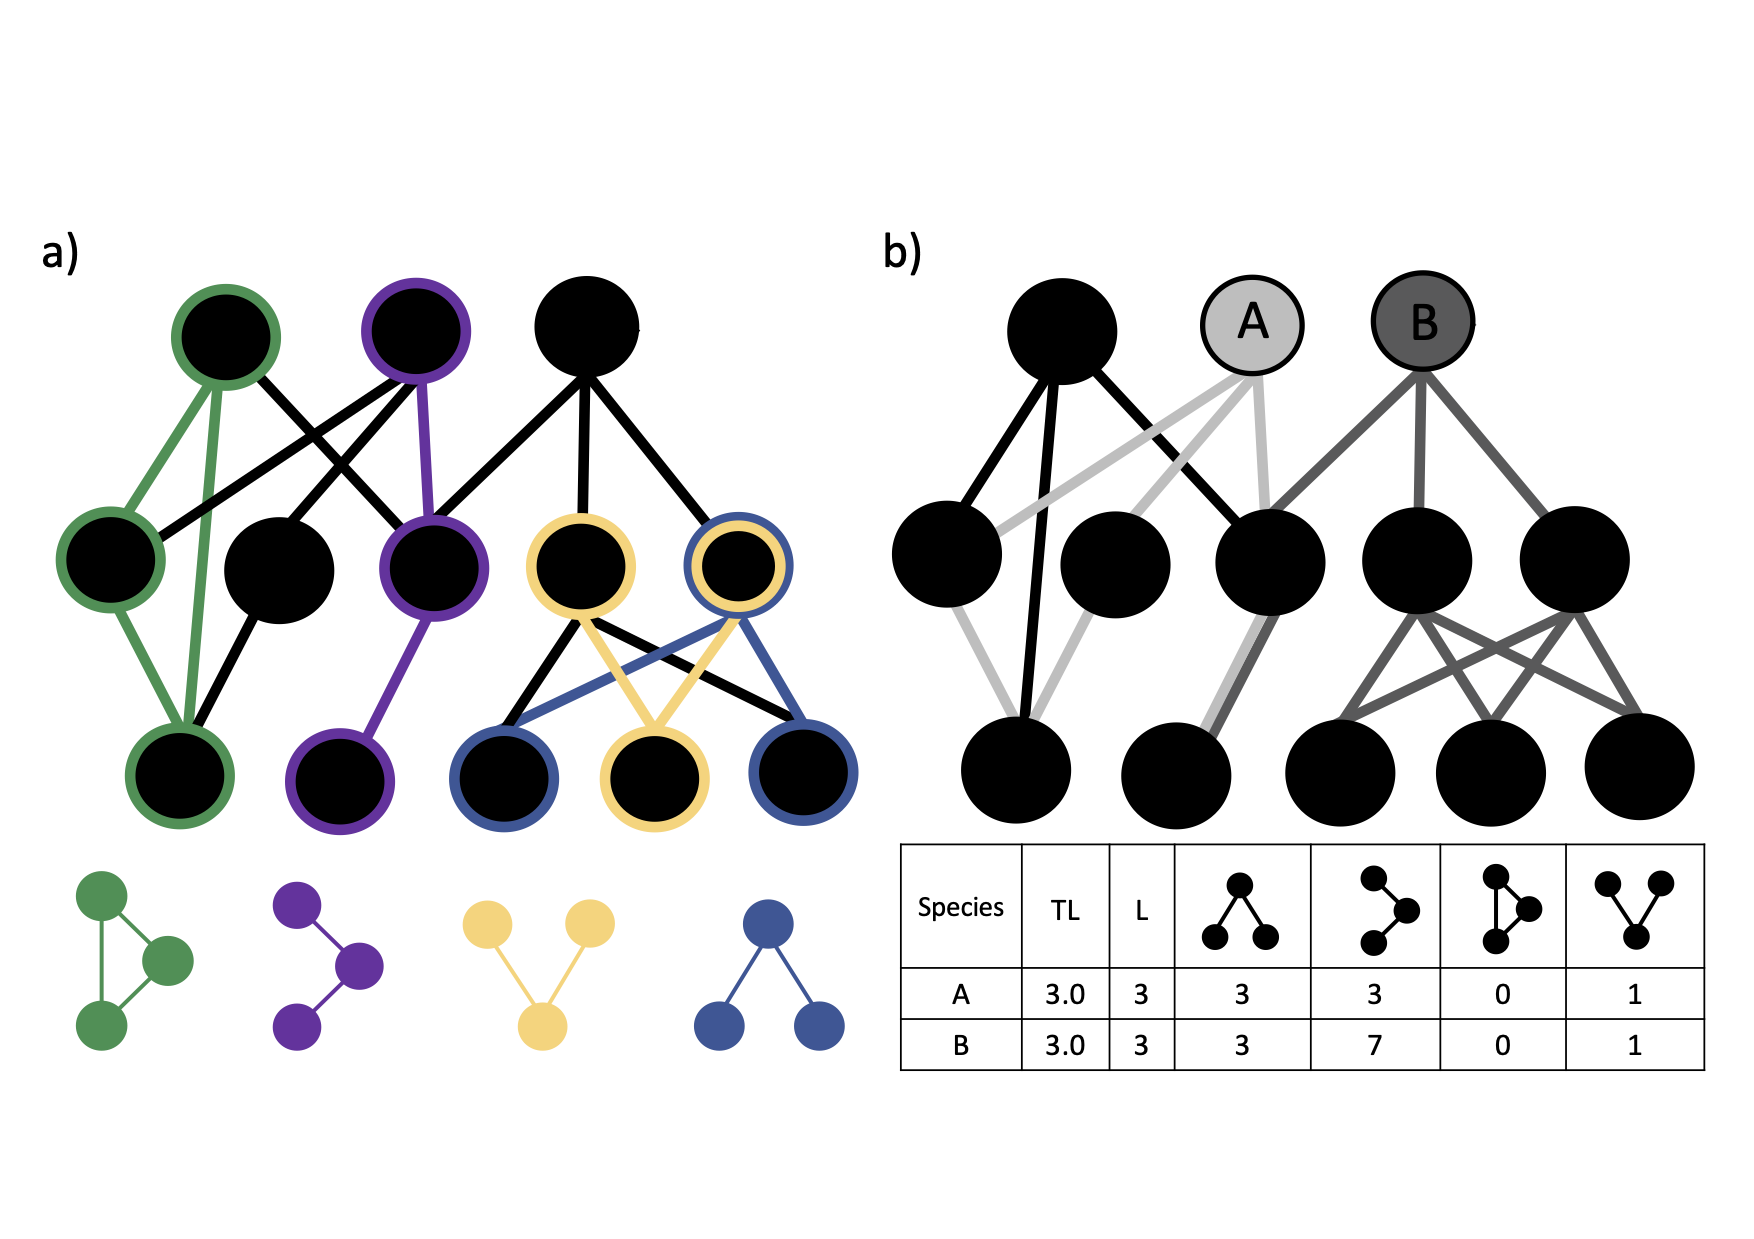
\includegraphics[width=1.0\textwidth]{manuscript/figures/concept_fig_ver2.png}
        \caption{Conceptual figure of a toy food web. \textbf{a)} This food web contains examples of the four motifs: apparent competition (blue), three-species chain (purple), omnivory (green), and direct competition (yellow). These motifs capture different ways in which disturbances to basal resources can propagate through the network. For example, a disturbance to the bottom species in a three-species chain will have a direct effect on the middle species but only indirectly affect the top species while a disturbance to the bottom species in an omnivory motif will have a direct effect on the middle species and direct and indirect effects on the top species. 
        Note that the nodes participate in more motifs than the ones highlighted. \textbf{b)} In the same food web, species with identical degree and trophic level can have different motif participation; here species A (light grey node with links in the same motif colored light grey) participates in only two chains while species B (dark grey node with its direct consumption links colored dark grey) participates in chains more than tree times more frequently (see inserted table for counts of participation in all four motifs). 
        Despite having equal degree and trophic level, species A may be at greater risk of going extinct than species B because of its dependence on specialist prey species. Two-thirds of the prey of species B are generalists and therefore more likely to survive a disturbance to basal resources. By including information about indirect interactions, motif profiles reflect this difference between species A and B while trophic level and degree do not.}
    \label{fig:concept}
    \end{figure}

    
        \begin{figure}[hb!]
        \centering
        \includegraphics[width=0.85\textwidth]{figures/persistence_vs_motifs.eps}
        \caption{The effect of proportion of the role (x-axis) made up by various motifs (columns) on persistence (y-axis). The effect of participating in each motif is based on the fixed effects in Equation~\ref{propreq}. The different colored lines indicate the probability of extinction of basal species, from $\pi_{disturbed} = 0.1$ (top, purple; no disturbance) to $\pi_{disturbed} = 0.5$ (bottom, yellow; high disturbance). 95\% confidence intervals for each line are shown in grey. Note that omnivory made up a smaller proportion of species' roles than other motifs; lines are plotted over the observed ranges of motif participation.}
    \label{fig:prop_lmer_all}
    \end{figure}
        

    \begin{figure}[hb!]
        \centering
        \includegraphics[width=\textwidth]{figures/roles_vs_TL.eps}
        \caption{Motif participation correlated with in-degree and trophic level, and both of these simpler role measures were also correlated with persistence. \textbf{A-B)} The proportion of omnivory increased with increasing degree while all other proportions decreased. The proportions of omnivory and direct competition decreased with increasing STL while the proportions of apparent competition and three-species chains increased. \textbf{C-D)} Persistence increased with increasing in-degree for low levels of disturbance to basal resources but decreased with increasing degree for high levels of disturbance to basal resources.
        Persistence declined with inceasing STL for all levels of disturbance to basal resources.}
        \label{fig:motifs_vs_TL_and_deg}
    \end{figure}        

    \begin{figure}[hb!]
    \centering
        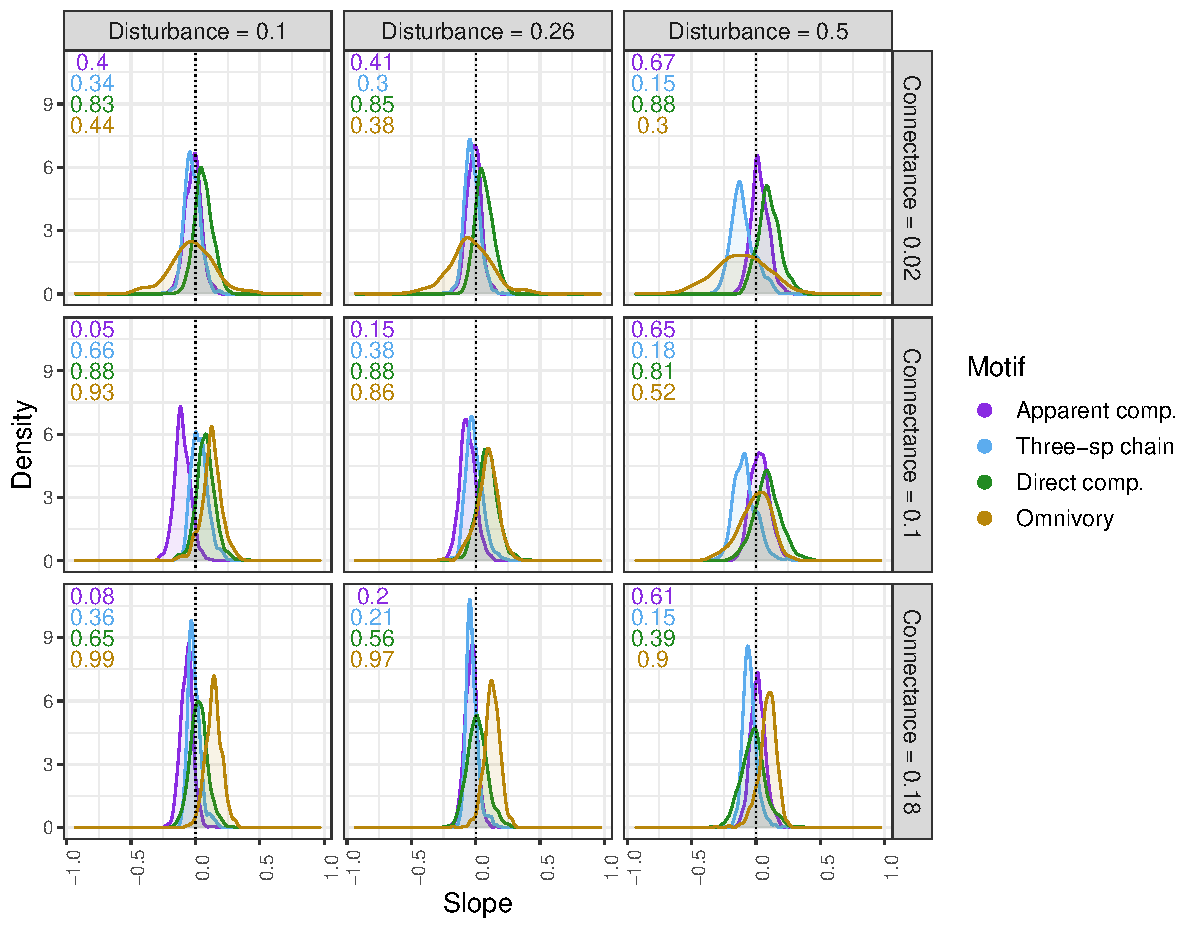
\includegraphics[width=\textwidth]{figures/prop_dens_bp_vs_C_allS.pdf}
        \caption{Here we show the density (y-axis) of slopes (x-axis) of persistence against proportion of different motifs for all simulated webs of all sizes - a visualization of how an increased proportion of each motif (different colored lines) affects persistence of consumer species. Columns show the result for various disturbances on the basal level, from $\pi_{disturbed} = 0.1$ (left) to $\pi_{disturbed} = 0.5$ (right). Rows show various levels of connectance. The dotted, vertical lines indicate zero on the x-axis. A negative slope value reflects a negative relationship between increased participation in a motif and persistence, while a positive slope value reflects a positive relationship - an increased proportion of a specific motif increases persistence. The fraction of replicates with a slope greater than zero are stated in numbers in each sub-plot, the color corresponding to each motif (legend). }
        \label{fig:density_prop_C}
    \end{figure}    
    
    \begin{figure}[hb!]
        \centering
        \includegraphics[width=\textwidth]{figures/persistence_motif_profiles.eps}
        \caption{The proportions of the four motifs in a network's motif profile are related to the mean persistence of species in the network. Specifically, persistence decreases as the proportion of omnivory in the network's motif profile increases while persistence increases with the proportions of the other three motifs. Interactions between motif profiles and disturbance were significant but small. Here we show the relationships of probabilities of extinction of basal resources of $\pi=0.1$ (top set of lines) and $\pi=0.5$ (bottom set of lines). Relationships are shown for the observed range of proportions for each motif.}      
        \label{fig:motif_profile_persistence}
    \end{figure}    
    
    \begin{figure}[hb!]
        \centering
        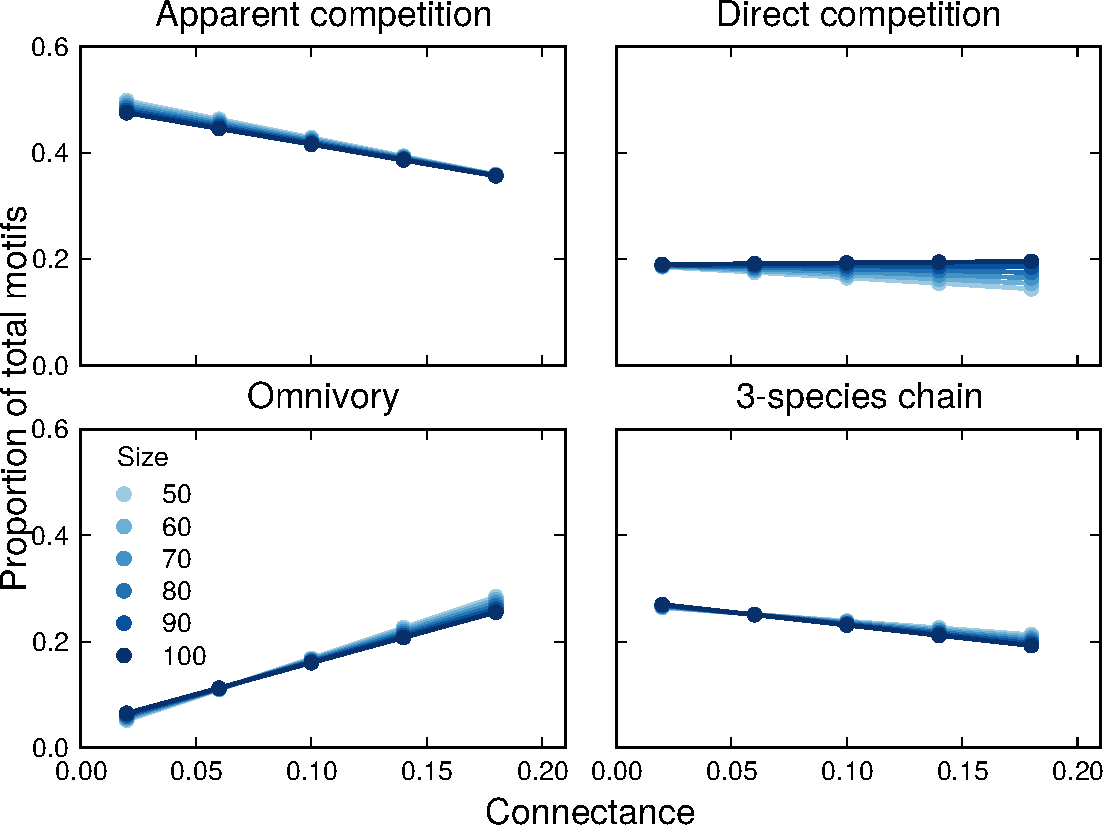
\includegraphics[width=\textwidth]{manuscript/figures/motif_proportion_lms.pdf}
        \caption{The proportions of the four motifs in a network's motif profile were related to network size, connectance, and their interaction. The effect of connectance was much stronger than the main effect or interaction with network size. The proportion of apparent competition in a network's profile decreased with increasing connectance, while the proportion of omnivory increased. In small networks, the proportion of direct competition also decreased with increasing connectance.}
        \label{motif_proportion_lms}
    \end{figure}

\clearpage

% \section*{Glossary}
% \begin{table}[h!]
% \label{glossary}
% \caption{Glossary of terms relating to motifs and Bayesian networks}
%     \footnotesize{
% \begin{tabular}{l|l}
%     Term & Definition \\
%     \hline
%     Motif & Set of $n$ interacting species. In this case, $n=3$ \\
%     Network motif profile & Vector describing the frequency of each motif in the network. \\
%     & Normalised by dividing counts of each motif by the total across all motifs.\\
%     Motif participation role & Vector describing the frequency with which a focal species appears in each motif.\\
%     & Normalised by dividing counts for each motif by the total across all motifs. \\
%     Bayesian network & A directed acyclic graph, used to predict species' likelihood of persistence. \\
%     Network persistence & The mean likelihood of consumers in a network not going extinct.\\
%     Species persistence & The individual likelihood of a species not going extinct.\\
%     In-degree & Number of prey species to a consumer species.\\
%     Trophic level (STL) & The shortest food chain between the focal species and any basal species.\\
%     Disturbance ($\pi_{disturbed}$) & Probability of extinction of a basal resource when extra disturbance is added. \\
%     Baseline extinction &  When no disturbance is applied, $\pi_{base}$=0.1.\\
% \end{tabular}}
% \end{table}

% Notes on what expressions and words to use
% "probability of extinction" or "level of disturbance" for the different disturbace scenarios?


\bibliographystyle{unsrtnat} 
\bibliography{anna_bib_new} % Abbreviate journal titles.

\end{spacing}

\end{document}

